%
% This is Chapter 2 file (chap2.tex)
%
\chapter{The Numerical Challenge} \label{chap2}

\section{Introduction}

In this chapter we first summarize both well-known and emerging
sources of numerical inaccuracy and describe techniques for supporting
reproducible accuracy. We then prove the inadequacy of conventional
wisdom when dealing with this problem and provide strong evidence of
the need for intelligent reduction operations at the extreme scale
before to conclude the chapter with a short summary of our our learned
lessons.

\section{Sources of Numerical Inaccuracy}
%\label{sec:sources}

Achieving reproducible numerical accuracy at exascale faces two
fundamental roadblocks: nonassociativity of floating-point arithmetic
and nondeterminism in the order by which operands are reduced.  In
this section, we provide an overview of the challenges that arise when
nonassociativity collides with nondeterministic reduction. To that
end, we discuss the primary mechanisms by which floating-point error
arises and propagates. We also summarize the existing body of work
addressing issues of nondeterminism at exascale.

\subsection{Nonassociativity: A Consequence of Finite Precision}

Floating-point computations suffer loss of accuracy, compared with the
same expression's evaluation in exact arithmetic, through two primary
mechanisms: alignment error and subtractive cancellation.  Alignment
error, by far the most common error modality, results from summation
of values whose exponents differ. Alignment error is possible whenever
two floating-point numbers that differ in magnitude by at least a
factor of two are added~\cite{Castaldo}. The amount of information
about the smaller operand lost due to alignment error is related to
the disparity between the operands' magnitudes. The other mechanism is
subtractive cancellation, which occurs when very small values are
obtained from the addition of two values with similar magnitude and
opposite sign. Subtractive cancellation, in contrast to alignment
error, is not a source of error \emph{per se}, but a means by which
inaccuracy in low-order mantissa bits of operands is transferred to
high-order mantissa bits of their sum.

A consequence of these inaccuracies is the well-known fact that
floating-point arithmetic operations are nonassociative, so the order
in which floating-point numbers are reduced via an operator (e.g., +,
-, *, /) influences the result.  For example, let $a = 10^9$, $b =
-10^{9}$, and $c = 10^{-9}$. In infinite precision, the summation
orders $(a + (b + c))$ and $((a+b) +c)$ are equivalent, but even in
double-precision floating-point arithmetic, the two distinct summation
orders yield different values.
\begin{center}
	$((a + b) + c) = ((10^9 - 10^9) + 10^{-9}) = 10^{-9}$ \\
	$(a + (b + c)) = (10^9 + (-10^9 + 10^{-9})) = 0$ 
\end{center}
For a small example such as this one, the flaw is clear, namely, that
the small-magnitude value $c$ is ``absorbed" by the much larger value
$b$.

\subsection{High Concurrency: A Consequence of Extreme Scale}

Contemporary petascale platforms consist of up to millions of
processor cores that must act in concert to effect large
simulations. Even at these scales, the cost of achieving not only
accuracy in floating-point reductions but reproducible accuracy is
felt. The scientific community at large has set its sights on
deployment of an exascale computing platform, and in response the HPC
community has identified a canonical set of challenges to implementing
an exascale machine~\cite{Doe2014}. Although emerging developments in
low-power hardware, advanced systems software, and algorithm design
show promise, it has become increasingly evident that achieving
reproducible numerical accuracy at exascale cannot rely on
deterministic reduction. Exascale computations will simply have to
weather perturbations in their reduction trees through algorithmic
means. In this section, we summarize key results demonstrating how
variability in reduction trees induces variability in sums of
floating-point numbers. Additionally, we present a set of findings,
commentary, and expert recommendations supporting our claim that
deterministic reduction trees at exascale will be unfeasible.

Throughout this section and the remainder of the chapter, we adopt the
view of a concurrent sum of floating-point numbers at the extreme
scale as a \emph{reduction tree}, which we define as a full binary
tree whose $N$ leaf nodes correspond to floating-point operands and
whose internal nodes correspond to the partial reductions formed in
the process of computing the final result--the root node.  Reduction
trees can vary in two ways: shape and assignment of operands to
leaves. When we refer to the shape of a reduction tree, we mean the
particular way in which nodes are linked by
edges. Figure~\ref{fig:redtree_diffshape} shows two differently shaped
reduction trees: a balanced (parallel) reduction tree and an
unbalanced (serial) reduction tree. For a fixed set of operands, even
two reduction trees with the same shape can yield different values for
the reduction if the assignment of operands to leaves differ between
the two trees.
\begin{figure}[!htb]
% \label{fig:redtree_diffshape}
\centering
%\minipage[t]{0.45\textwidth}
%\begin{tabular}{c}
\subfigure[A balanced (parallel) reduction tree]{
%{.5\textwidth}
\centering
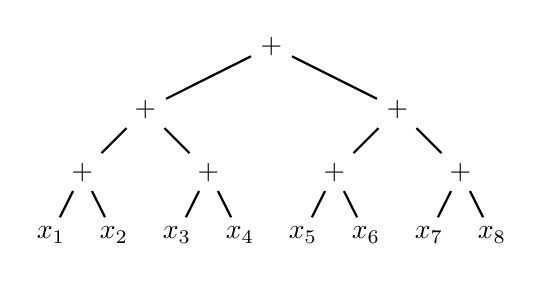
\begin{tikzpicture}[scale=0.8]
	\node at (0, 0) (1) {$x_1$};
	\node at (1, 0) (2) {$x_2$};
	\node at (2, 0) (3) {$x_3$};
	\node at (3, 0) (4) {$x_4$};
	\node at (4, 0) (5) {$x_5$};
	\node at (5, 0) (6) {$x_6$};
	\node at (6, 0) (7) {$x_7$};
	\node at (7, 0) (8) {$x_8$};
	\node at (.5, 1) (11) {$+$};
	\node at (2.5, 1) (12) {$+$};
	\node at (4.5, 1) (13) {$+$};
	\node at (6.5, 1) (14) {$+$};
	\node at (1.5, 2) (21) {$+$};
	\node at (5.5, 2) (22) {$+$};
	\node at (3.5, 3) (top) {$+$};
	\draw [draw=black, thick] (1)--(11)--(2);
	\draw [draw=black, thick] (3)--(12)--(4);
	\draw [draw=black, thick] (5)--(13)--(6);
	\draw [draw=black, thick] (7)--(14)--(8);
	\draw [draw=black, thick] (11)--(21)--(12);
	\draw [draw=black, thick] (13)--(22)--(14);
	\draw [draw=black, thick] (21)--(top)--(22);
\end{tikzpicture}
\label{redtree_balanced}}
\subfigure[An unbalanced (serial) reduction tree]{
\centering
	\begin{tikzpicture}[scale=0.8]
	\node at (-2, 0) (empty) { };
	\node at ( 4, 0) (empty) { };
	\node at (0, 0) (1) {$x_1$};
	\node at (1, 0) (2) {$x_2$};
	\node at (.5, 1) (11) {$+$};
	\node at (1.5, 1) (12) {$x_3$};
	\node at (1, 2) (21) {$+$};
	\node at (2, 2) (22) {$x_4$};
	\node at (1.5, 3) (31) {$+$};
	%\node at (2.5, 3) (32) {$x_5$};
	%\node at (2, 4) (41) {$+$};
	%\node at (3, 4) (42) {$x_6$};
	%\node at (2.5, 5) (51) {$+$};
	%\node at (3.5, 5) (52) {$x_7$};
	%\node at (3, 6) (61) {$+$};
	%\node at (4, 6) (62) {$x_8$};
	%\node at (3.5, 7) (top) {$+$};
	\draw [draw=black, thick] (1)--(11)--(2);
	\draw [draw=black, thick] (11)--(21)--(12);
	\draw [draw=black, thick] (21)--(31)--(22);
	%\draw [draw=black, thick] (31)--(41)--(32);
	%\draw [draw=black, thick] (41)--(51)--(42);
	%\draw [draw=black, thick] (51)--(61)--(52);
	%\draw [draw=black, thick] (61)--(top)--(62);
	\end{tikzpicture}
\label{redtree_unbalanced}}
\caption{Two reduction trees at the opposite ends of the spectrum.}
\label{fig:redtree_diffshape}
\end{figure}

The effect of varying reduction tree shape and varying operand-to-leaf
assignment is explored in~\cite{chiang13}. In their work, a set of
eight identical floating-point values is summed via three differently
shaped reduction trees, yielding in each case a different value for
the sum. Another set of eight floating-point values, six small and two
large, is summed via three reduction trees of the same shape, but with
different assignments of summands to leaves. Again, all three computed
sums disagreed.  One key observation is that the consequences of
nondeterministic reduction and floating-point nonassociativity are
felt even for extremely small examples.

On exascale systems the high level of concurrency will not allow the
user to enforce any specific reduction order because doing so is
either too expensive or impossible. At the same time variability in
floating-point error accumulation may become so great that debugging
is impaired or, worse, fundamentally incorrect results are
accepted. An exascale algorithm must exploit the extreme level of
concurrency, minimize communication (for speed and power reduction),
tolerate frequent hardware failures, and utilize resources as they
become available~\cite{Doe2014}, all the while providing some trust in
the computation's result.

The conflict between achieving reproducible accuracy and achieving
performance is primarily due to the fact that even on current HPC
platforms, communication costs dominate arithmetic costs.  Simply put,
the most performant reduction trees are those that take into account
the underlying physical topology of the system, which means reducing
values in an order based on which core produced them, not necessarily
their arithmetical properties. Conversely, the reduction trees that
result in the least error accumulation reduce values based on their
arithmetical properties, not their position in the topology of the
system. Recently, Balaji and Kimpe~\cite{balaji13} showed not only
that topology-aware reduction trees for MPI collective operations
outperform fixed-reduction trees but that the performance advantage of
allowing the reduction tree to conform to the system topology, as
opposed to a specified ordering of partial reduction, increases with
the number of cores.

\section{Mathematical Techniques}
%\label{sec:techniques}

In response to the challenges posed by the nonassociativity of
floating-point summation and the nondeterminism at the extreme scale,
mathematical techniques can be applied to mitigate the degree to which
computed sums exhibit sensitivity to reduction order. Lower
sensitivity results in increasingly reproducible results.  Techniques
can range from simple fixed-reduction orders to more sophisticated
prerounded algorithms. In this section we provide a general overview
of the techniques; however, in the rest of the chapter, we consider only
the compensated summation algorithms (Kahan and composite precision)
as well as the prerounded algorithms for our studies because they are
the only methods that can be feasibly applied at the exascale.

\subsection{Fixed-Reduction Order}

To apply fixed-reduction order, we need to ensure that all
floating-point operations are evaluated in the same order from run to
run. Two major problems exist for this strategy. The obvious problem
is that ensuring that the reduction proceeds according to a
user-determined reduction tree incurs massive communication and
synchronization costs.  Additionally, determining exactly which
reduction tree achieves minimal error for a given set of summands is
nontrivial. Conventional wisdom suggests summing the values in
ascending order if they all have the same sign, and in descending
order of magnitude if they are not. The first case is rare, however,
and the second case assumes that no error beyond initial
representation error is present in the summands; otherwise it is far
more vulnerable to catastrophic cancellation.  In summary, fixing the
reduction order is difficult to do correctly where it is possible, but
the salient point is that it cannot be done in a cost-effective way at
exascale~\cite{Demmel_Hida}.

\subsection{Interval Arithmetic}

Techniques based on interval arithmetic replace floating-point types
with custom types representing finite-length intervals of real
numbers. The actual value of the reduction is guaranteed to lie within
the interval. The width of the interval increases with the uncertainty
of the computation. While the techniques are reproducible by design,
they also cause large slowdown and are not suitable for applications
needing many digits of accuracy.

\subsection{High-Precision Arithmetic}

Perhaps the most obvious technique, and certainly the most popular in
real applications, is to use higher-precision floating-point types. To
our knowledge, the earliest work directly addressing the issue of
numerical reproducibility~\cite{he} demonstrates the use of the
double-double precision floating-point type in a critical section of
code to curtail variability in a global sum. In that work, the goal of
using multiple floating-point types was explicitly to achieve
reproducible results. Parallel to that effort, significant progress
has been made in the field of automated floating-point precision
tuning (e.g., ~\cite{precimonious}). Precision tuning is an attempt
to reduce precision where possible while maintaining a prescribed
degree of accuracy.  While one can achieve greater
reproducibility by pursuing greater accuracy, the use of
high-precision arithmetic can result in memory-demanding
algorithms. By increasing the size of floating-point variables in most
numerically sensitive parts of the algorithm, for example with manual
changes made by an expert or by some form of analysis, we can reduce
the memory requirements. Still the technique relies on either human
experts or other software and thus is probably unsuitable for many 
of the use cases discussed in the recent DOE exascale
report~\cite{Doe2014}.

\subsection{Compensated Summation Algorithms}

To compute the sum of $n$ values, we obtain $n-1$ partial sums in the
process. For each of these partial sums, the magnitude of error can be
estimated.  Based on that estimate, an attempt can be made to
compensate for that error by adding an error term to each partial
sum. Compensated summation is a relatively old technique, having been
introduced by Kahan in~\cite{kahan65}; but families of more
sophisticated compensated summation algorithms have been developed,
such as composite precision (CP) summation~\cite{Taufer2010}. In
Kahan's algorithm the estimated error is added back into the sum at
each step. In CP, the error summation is kept and propagated as each
of the summations are performed and added back in only at the end.

\subsection{Prerounded Summation Algorithms}

More recently, an approach called prerounded summation has emerged for
reproducible and accurate summation.  The common strategy used by this
type of algorithm is splitting the operands into ``high-order" and
``low-order" parts with the property that the high-order parts can be
summed irrespective of summation order and the low-order parts can be
neglected, or recursed upon, for higher accuracy. The algorithms
proposed by Demmel and his group are integrated into the ReproBLAS
library~\cite{demmel}, which at this time is undergoing active
development.

\section{Inadequacy of Conventional Wisdom}

The management of reproducible numerical accuracy is closely related
to the task of estimating and predicting error accumulation.  Three
common approaches exist, typically used in isolation, to quantify and
mitigate error accumulation. Two of the approaches can be broadly
classified as techniques for error estimation: using worst-case error
bounds and attempting to track or avoid subtractive cancellation. The
third approach is the use of summation algorithms that are believed to
be inherently less sensitive to variability in the reduction tree.  We
emphasize that these approaches have significant value. However, we
demonstrate that the use of any one approach, in isolation, will not
guarantee the reproducibility desired without a potentially
significant loss of performance.

\subsection{Using Analytical Error Bounds}

The analysis of the error for a single floating-point sum can be
extended to produce a worst-case error bound for the reduction of
multiple floating-point values.  For IEEE-compliant implementations of
floating-point arithmetic, we have the following bound on the roundoff
error for a single operation. Let $x, y$ be floating-point numbers,
let $\texttt{fl}(x+y)$ be their rounded sum according to a given
rounding rule, and let $(x+y)$ be their exact sum:
\begin{center}
	$\texttt{fl}(x+y) = (x+y)\cdot (1+\delta)$ 
\end{center}
where $|\delta| \leq u$ where $u$ is the unit-roundoff and may be
written $u = \frac{1}{2}\beta^{1-p}$, where $\beta$ is the base and
$p$ is the number of mantissa bits of the representation of $x$ and
$y$. Equivalently, if we let $z$ denote the exact sum $x+y$, we obtain
a bound on the absolute error $| \texttt{fl}(x+y) - z| \leq u$.  With
some algebra, one can prove an upper bound on the error in a sum of
$n$ floating-point numbers. We do not include the proof here (it may
be found in~\cite{Higham93}), but we state the result. Let $x_1,
\ldots, x_n$ be floating-point numbers, let $z$ denote their exact
sum, and let $\sum\limits_{i=1}^{n}x_i$ denote their sum in
floating-point arithmetic. Then we have the following upper bound on
the absolute error in the sum:
\begin{center}
	$|\sum\limits_{i=1}^{n}x_i - z| < n \cdot u \cdot \sum\limits_{i=1}^{n} |x_i|.$
\end{center}

%While this upper bound is useful in the sense that it is better than
%nothing, it is excessively loose in practice.  We present the
%analysis for a single sum, the extension to a sum of $N$ values, and
%data demonstrating the looseness of the bound.  Unlike arithmetic
%over the real numbers, arithmetic with floating-point operands
%suffers from some limitations. Due to the availability of a finite
%number of bits to represent each number, the vast majority of real
%numbers do not have an exact representation in a given system of
%floating-point arithmetic. Consequently, when two floating point
%values are summed, the result must often be rounded according to some
%rounding rule. The difference between this rounded result and the
%exact result had the summation been conducted over the real numbers
%is what we refer to as roundoff error.  In practice however, we are
%more interested in bounds on the error that accumulates over the
%course of summing $n$ floating-point values.

Using analytical or statistical worst-case error bounds causes
overestimation of the errors. Figure~\ref{fig:errorbounds} shows an
empirical case study in which we measure the error magnitudes for
$10,000$ values sampled in the range $(-1000, +1000)$ and summed by
using $10,000$ different summation orders.
\begin{figure}[!htb]
  \centering
  \includegraphics[width=0.80\textwidth]{chapter_2_figures/error_variability_histogram.pdf}
  \caption{Empirical study of error magnitudes and worst-case error
    bounds for $10,000$ summations of $10,000$ values randomly
    sorted.}
  \label{fig:errorbounds}
\end{figure}
The figure also shows both the analytical and statistical worst-case
error bounds. Both error bounds significantly overestimate the error
magnitude. At the same time we observe the large range of measured
errors obtained for the same set of values just by randomly shuffling
the order in which the terms are summed.

\subsection{Tracking Cancellations}

When considering sets of summands with both positive and negative
values, the potential for \emph{catastrophic cancellation} arises in
the computation of the sum. This numerical phenomenon can result in
large relative errors in both the partial and final sums, leading to
the intuitively appealing perspective of achieving reproducible
accuracy by structuring reductions to avoid cancellation.

Cancellation in general refers to the scenario where the sum of two
floating-point values has a smaller exponent than both of the
summands. In order to subtract one floating-point number from another,
their binary points are aligned and the mantissa of their difference
is determined by subtracting the mantissas of the operands bitwise and
then \emph{renormalizing} the result. The effect of the
renormalization process is that the lower-order bits of the operands
determine the higher-order bits of the result. If both summands are
exact in the sense that their mantissa bits are not carrying the error
from previous computations---as is almost never the case---then their
difference can be considered accurate. However, if the low-order bits
of the operands are inaccurate due to alignment error, many or all of
the mantissa bits of the difference of the operands may be
inaccurate. This is the ``catastrophic" case.

We emphasize, however, that cancellation does not in and of itself
cause error to accumulate. Rather, it reveals error that has already
accumulated in the operands. In a sense, relative error can increase
because of catastrophic cancellation as uncertainty in
less-significant bits of the operands' mantissas is transferred to
uncertainty in the most significant bits of the result's
mantissa. Nevertheless, the number of cancellations is not a reliable
indicator of the overall problem.

To prove this claim, we generate a counterexample with a set of
$1,000$ floating-point numbers uniformly distributed in $[-1, 1]$.  We
compute the sum of these numbers using 100 distinct summation orders
and determine the error for each order. We assess cancellation for
each order using the numerical library CADNA~\cite{jezequel}. CADNA
uses the CESTAC method to identify instances of cancellation in a sum
and, for each instance, estimate the difference between the number of
accurate digits in the operands and the number of accurate digits in
the result. In this sense, a cancellation resulting in the loss of
four digits of accuracy is more severe than a cancellation resulting
in the loss of only two digits. Figure~\ref{fig:errorcancellations}
shows the cancellation counts and error magnitudes for several
summation orders of the set of interest for our counterexample. Each
summation order is represented by five bars, four showing the number
of cancellations resulting in the loss of one, two, four, and eight
digits, respectively, and a fifth bar showing the error magnitude,
scaled for ease of viewing. We observe that the number of
cancellations, at any of the considered severities, does not
consistently predict error magnitude.  In particular, consider
summation orders 2 and 4. Order 2 has about 5X as many digit
cancellations as order 4, but only half the error. This result lends
credence to the view that although it is tempting to view ``keeping
track of cancellations" as a valid strategy for managing error and
ensuring reproducibility, there is not a simple correspondence between
instances of cancellation and error magnitude. Rather, the
relationship between cancellation and error depends on knowledge of
how much error has already accumulated in the operands involved in the
cancellation, a quantity whose estimation is impeded by the previously
discussed loose error bound.
\begin{figure}[!htb]
  \centering
  \includegraphics[width=0.80\textwidth]{chapter_2_figures/cancel_chart.pdf}
  \caption{Empirical study of cancellations vs. error magnitude
    for different summation orders.}
  \label{fig:errorcancellations}
\end{figure}

\subsection{Choice of Summation Algorithm}

Apart from the standard iterative summation algorithm, we examine
other summation algorithms that exhibit reduced sensitivity to
variability in the reduction tree. However, each of these algorithms
incurs a certain performance penalty relative to the standard
summation. Standard summation is the cheapest and least
complex. Kahan's compensated summation, then composite precision
summation, and finally prerounded summation are expected to
progressively provide more accuracy at the expense of performance. To
assess this performance impact, we measure the execution times of a
case study designed to emulate scenarios in scientific computing in
which partial data is locally generated on multiple processes and then
is globally reduced across the processes. Specifically, on each
process, we generate a chunk of a vector of values of length $10^6$
from a series that is known to sum to zero under exact arithmetic. We
locally reduce these values using each of the four summation
algorithms: in the case of Kahan and composite precision, we use the
summation operators in~\cite{Robey2011} and in the case of prerounded
summation, we use the dIAddd operator provided
in~\cite{reproblas}. Finally, we globally reduce the local sums by
using MPI\_Reduce with custom reduction operators for Kahan, composite
precision, and prerounded summations. To avoid time variations due to
network contention we run our tests on a single dedicated 48-core AMD
node. Each tests is repeated 20 times with a warmed
cache. Figure~\ref{fig:compare_runtimes} shows the average execution
times and Figure~\ref{fig:compare_ratios} shows the performance
penalties associated with more-reproducible summation. The latter
figure confirms the proposed ranking of the summation algorithms in
terms of performance expense.
\begin{figure}[!htb]
    \centering
    \includegraphics[width=0.80\textwidth]{chapter_2_figures/runtimes.pdf}
    \caption{Comparison of execution time to sum $10^6$ terms for
      standard summation (ST), Kahan's compensated summation (K),
      composite precision summation (CP), and prerounded summation
      (PR).}
    \label{fig:compare_runtimes}
\end{figure}
\begin{figure}[!htb]
    \centering
    \includegraphics[width=0.80\textwidth]{chapter_2_figures/ratios.pdf}
    \caption{Performance losses of Kahan's compensated summation (K),
      composite precision (CP), and prerounded (PR) summations
      compared to the standard summation (ST).}
    \label{fig:compare_ratios}
\end{figure}

%Empirical results obtained on a single 48-core AMD node
%of a dedicated cluster support this characterization. Specifically,
%performance analysis of the four algorithms indicates that the
%execution time needed to reduce a vector $10^6$ elements increases
%with the reproducible accuracy provided by the algorithm as shown in
%Figure~\ref{fig:compare_runtimes}. Figure~\ref{fig:compare_ratios}
%shows the performance losses of the enhanced sums (i.e., Kahan's
%compensated summation, composite precision summation, and prerounded
%summation) which agree with previous empirical
%results~\cite{demmel}~\cite{Taufer2010}.

We argue that applying a judicious mixture of these algorithms, as
opposed to uniformly applying a single technique, is necessary for
achieving numerical reproducibility to the degree required by an
application, for a cost acceptable for that application.
Figures~\ref{fig:avgalgorithms}(a) and~\ref{fig:avgalgorithms}(b)
support this claim by showing the relative sensitivity of the three
summation algorithms: Kahan's compensated summation (K), composite
precision summation (CP), and prerounded summation (PR).  For a fixed
set of data we generate multiple reduction trees of the same shape but
with different assignments of operands to leaves. We construct the set
of summands to have mathematical properties that render its reduction
especially prone to both alignment error and loss of accuracy due to
cancellation. For each reduction tree, we compute the sum using each
of the four algorithms. By plotting the error magnitude, we see that
as a progressively greater amount of computation is invested in
compensating for roundoff error, the sum becomes less sensitive to the
varying reduction tree.
\begin{figure}[!htb]
\centering
\minipage[t]{0.40\textwidth}
\begin{tabular}{c}
\includegraphics[width=\textwidth, height=8cm]{chapter_2_figures/draft_boxplot_alt_balanced_N=1048576.pdf} \\ 
(a) \\
\end{tabular}
\endminipage
\minipage[t]{0.30\textwidth}
\begin{tabular}{c}
\includegraphics[width=\textwidth, height=8cm]{chapter_2_figures/draft_boxplot_balanced_cp_vs_preround_N=1048576.pdf}
\\ (b) \\
\end{tabular}
\endminipage
\caption{Empirical study of relative sensitivity of three summation
  algorithms: Kahan's compensated summation (K), composite precision
  summation (CP), and prerounded summation (PR). Note that (a) zooms
  into (b). }
\label{fig:avgalgorithms}
\end{figure}

\section{Exploring the Reproducibility Space} 

Previous work~\cite{chiang13, balaji13} found that reduction tree
shape and assignment of operands to its leaves (or threads) can have a
profound effect on the concurrent sum of $n$ floating-point numbers,
even when the operands themselves are subject to minimal alignment
error and have the same sign avoiding cancellation.  We build the work
in this chapter on this previous work by targeting a much larger
reduction scale and investigating the impact of four independent
parameters on the variability of a sum when the reduction order is
non-deterministic. The four parameters we consider are the condition
number, the dynamic range, the level of concurrency, and the reduction
algorithm. We present three kinds of results. First, we examine the
sensitivity to variations in the reduction tree of four summation
algorithms at increasing levels of concurrency. Second, we study the
impact of concurrency, condition number, and dynamic range on
reproducible numerical accuracy. Third, we provide evidence of the
need for selecting application-aware reduction algorithms.

\subsection{Experimental Environment and Parameters}

Building on the results of small nondeterministic reduction trees
established in~\cite{chiang13, langlois}, we consider reduction trees
at the size expected for exascale systems consisting of floating-point
operands reflective of those actually reduced in simulations. Since an
exascale system is not available, we emulate the reduction process
with $n$ threads, each computing one of the $n$ partial sums.  We
consider two tree shapes at opposite ends of the spectrum: a
completely balanced (see Figure~\ref{redtree_balanced}) tree and a
completely unbalanced (see Figure~\ref{redtree_unbalanced}) tree.  For
each tree shape, we generate distinct reduction trees by randomly
assigning operands to leaves. We also focus on sets of floating-point
summands whose mathematical properties are less amenable to
reproducible summation. We characterize sets of floating-point values
by their sum condition number and dynamic range. These are intrinsic
properties of the set of values; they are independent of any imposed
ordering. For a set of floating-point numbers $\{x_1, \ldots, x_n
\}$, the sum condition number is defined as
\[k = \left(\sum_{i=1}^{n}|x_i|\right)/\left|\sum_{i=1}^{n}x_i\right|\] and
the dynamic range is defined as
\begin{center}
	$dr = \texttt{exp}(\texttt{max}(|x_i|))-\texttt{exp}(\texttt{min}(|x_i|)),$
\end{center}
where $exp(x)$ is the value of the exponent in the representation of
$x$.  If the dynamic range of two numbers is larger than zero, then
alignment error will occur. For this reason, we use the dynamic range
of a set of values as a rough estimator of alignment error.  The
condition number does not correspond to a single mechanism by which
error accumulates.  Instead, it describes how sensitive the final sum
is to small errors in the partial sums.

Table~\ref{tab:parameters} shows small sample sets of values
presenting dynamic range $dr$ equal to 0, 8, and 16 as well as
condition number $k$ equal to 1, 1000, and $\infty$.  Note that $dr$
equal to $0$ means ``all exponents are the same'' and not that the
numbers are large or small; on the other hand a larger $dr$, for
example 8 or 16, means that a larger discrepancy exists between the
largest and smallest exponents. In other words, the sign on the
summands makes no difference, and the sum of summands makes no
difference. A condition number equal to 1 means ``all values in sum
have the same sign,'' while a condition number number infinity means
``the sum of all the values is 0.''
\begin{table}[!ht]
\caption{Example of sample set of values with specified dynamic range,
  $dr$, and condition number, $k$.}
\label{tab:parameters}
\center
\small
\begin{tabular}{|c|c|c|}
  \hline
  Sample Set of Values & $dr$ & $k$ \\
  \hline
  $\{$1.23e+32, 1.35e+32, 2.37e+32, 3.54e+32$\}$ & $0$ & $1$ \\
  $\{$1.23e-32, 1.35e-32, 2.37e-32, 3.54e-32$\}$ & $0$ & $1$ \\
  $\{$-1.23e+16, -1.35e+16, -2.37e+16,-3.54e+16$\}$ & $0$ & $1$ \\
  $\{$2.37e+16, 3.41e+8, 4.32e+8, 8.14e+16$\}$ & $8$ & $1$ \\
  $\{$3.14e+32, 1.59e+16, 2.65e+18, 3.58e+24$\}$ & $16$ & $1$ \\
  \hline
  $\{$2.505e+2, 2.5e+2, -2.495e+2, -2.5e+2$\}$ & $0$ & $1000$ \\
  $\{$5.00e+2, 4.99999e-1, 1.0e-6, -4.995e+2$\}$ & $8$ & $1000$ \\
  $\{$5.00e+2, 4.99...99e-1, 1.0e-14, -4.995e+2$\}$ & $16$ & $1000$ \\
  \hline
  $\{$3.14e+8, 1.59e+8, -3.14e+8, -1.59e+8$\}$ & $0$ & $\infty$ \\
  $\{$3.14e+4, 1.59e-4, -3.14e+4, -1.59e-4$\}$ & $8$ & $\infty$ \\
  $\{$3.14e+8, 1.59e-8, -3.14e+8, -1.59e-8$\}$ & $16$ & $\infty$ \\
  \hline
\end{tabular}
\end{table}
\normalsize In~\cite{chiang13} the operands are well-conditioned; they
have $k=1$ (the best possible condition number) and, when varying tree
shape, have $dr=0$. We instead focus on ill-conditioned inputs with
high dynamic range because reality is not so rosy. For example,
$N$-body simulations~\cite{bailey} involve reductions of
floating-point values that are ill-conditioned; both $k$ and $dr$ can
frequently be very large.

\subsection{Sensitivity of Summation Algorithms}

To examine the sensitivity of summation algorithms to variability in
the reduction tree, we generate and reduce two sets of summands
constructed to have the exact sum of zero and dynamic range of
$32$. One set has $n=8K$ values, and the other has $n=1M$ values.
These sets of values are more prone to both alignment error and
catastrophic cancellation than are those studied in~\cite{chiang13}.
They are also more reflective of the values that may arise in
simulations (e.g., when the net force on a particle is close to zero).

Figures~\ref{fig:boxplot}(a)--(h) show the distribution of error
magnitudes for sums computed by using varying reduction trees for the
four summation algorithms of interest in this chapter: the standard
iterative summation algorithm (ST); Kahan's compensated summation
algorithm (K); the composite precision summation (CP), which can be
considered an enhanced form of compensated summation; and the
prerounded summation (PR), which offers guaranteed bitwise
reproducibility at a user-specified level of accuracy. We consider two
types of reduction trees: completely balanced, with results shown in
Figures~\ref{fig:boxplot}(a), (b), (c), and (d), and completely
unbalanced, with results shown in Figures~\ref{fig:boxplot}(e), (f),
(g), and (h). For each tree type, we consider both smaller levels of
concurrency (8K leaves in the tree) and higher levels (1M leaves in
the tree). The boxplots in the figures are obtained by considering 100
distinct reduction trees with the same shape but randomly permuted
assignments of the values to leaves. Note that
Figures~\ref{fig:boxplot}(b), (d), (f), and (h) provide a zoom-in into
Figures~\ref{fig:boxplot}(a), (c), (e), and (g), respectively.
\begin{figure*}[!htb]
\centering
\minipage[t]{0.40\textwidth}
\begin{tabular}{c}
\includegraphics[width=\textwidth,
  height=4cm]{chapter_2_figures/draft_boxplot_balanced_N=8192.pdf} \\ (a)
Balanced, n=8K \\
\end{tabular}
\endminipage 
\minipage[t]{0.30\textwidth}
\begin{tabular}{c}
\includegraphics[width=\textwidth,
  height=4cm]{chapter_2_figures/draft_boxplot_balanced_cp_vs_preround_N=8192.pdf}
\\ (b) Zoom into (a) \\
\end{tabular}
\endminipage 
 \\
\minipage[t]{0.40\textwidth}
\begin{tabular}{c}
\includegraphics[width=\textwidth, height=4cm]{chapter_2_figures/draft_boxplot_balanced_N=1048576.pdf} \\
(c) Balanced, n=1M\\
\end{tabular}
\endminipage 
\minipage[t]{0.30\textwidth}
\begin{tabular}{c}
\includegraphics[width=\textwidth, height=4cm]{chapter_2_figures/draft_boxplot_balanced_cp_vs_preround_N=1048576.pdf} \\
(d) Zoom into (c)\\
\end{tabular}
\endminipage 
 \\
\minipage[t]{0.40\textwidth}
\begin{tabular}{c}
\includegraphics[width=\textwidth, height=4cm]{chapter_2_figures/draft_boxplot_unbalanced_N=8192.pdf} \\
(e) Unbalanced, n=8K \\
\end{tabular}
\endminipage
\minipage[t]{0.30\textwidth}
\begin{tabular}{c}
\includegraphics[width=\textwidth, height=4cm]{chapter_2_figures/draft_boxplot_unbalanced_cp_vs_preround_N=8192.pdf} \\
(f) Zoom into (e)\\
\end{tabular}
\endminipage 
 \\
\minipage[t]{0.40\textwidth}
\begin{tabular}{c}
\includegraphics[width=\textwidth, height=4cm]{chapter_2_figures/draft_boxplot_unbalanced_N=1048576.pdf} \\
(g) Unbalanced, n=1M\\
\end{tabular}
\endminipage 
\minipage[t]{0.30\textwidth}
\begin{tabular}{c}
\includegraphics[width=\textwidth, height=4cm]{chapter_2_figures/draft_boxplot_unbalanced_cp_vs_preround_N=1048576.pdf} \\
(h) Zoom into (g)\\
\end{tabular}
\endminipage 
  \caption{Error distributions for the four summation algorithms
    considered in this chapter for balanced and unbalanced reductions:
    three at a smaller (8K leaves) and one at higher (1M leaves)
    levels of concurrency.}
\label{fig:boxplot}
\end{figure*}

The effect of nondeterminism in the reduction tree is exhibited in
Figures~\ref{fig:boxplot}. For a given summation algorithm, the
distribution of data points and width of the box indicate how much the
sum tends to vary when the overall shape of the reduction tree is
constant but the arrangement of summands to its leaves is
variable. Within the subfigures, we see that although Kahan summation
tends in general to produce more reproducible sums than standard
summation, only composite precision and prerounded summations offer
reproducible numerical accuracy at an acceptable level.  Across a row
of subfigures, we see that as the level of concurrency rises, the
absolute error in the sum rises as expected. However, by comparing
results across a column of subfigures, for example, the ST data from
Figure~\ref{fig:boxplot}(a) and the ST data from
Figure~\ref{fig:boxplot}(e), we see that much more variation in the
sum occurs when the tree is unbalanced than when it is balanced for
the standard summation algorithm. To cope with intermittent faults and
inconsistently available resources, we expect that the reduction trees
employed by an exascale system will vary not only in terms of
arrangement of data among their leaves but also in overall shape. We
conclude that because of the difference in reproducibility observed
for differently shaped reduction trees, exascale applications will
need to maintain awareness of the degree of fluctuation in reduction
tree shape and employ more robust reduction operators accordingly.

\subsection{Effect of Concurrency, Conditioning, and Dynamic Range}

For a fixed level of concurrency, the mathematical properties of the
summands can have a significant impact on the sensitivity of the sum
to variations in the reduction tree. In the previous section, we
considered a set of values with a fixed condition number $k$ and
dynamic range $dr$.  In this section, we examine the effects of
varying $k$ and $dr$ at a fixed level of concurrency $n=1M$; varying
$dr$ and $n$ at a fixed $k$; and varying $k$ and $n$ at a fixed
$dr$. We represent the spaces of $(k, dr)$, $(n, dr)$, and $(n, k)$ as
a grid of cells, where for each cell we generate a set of
floating-point values with the cell parameters. The degree to which
these sets of values can be summed reproducibly is tested. For all
sets of summands under consideration, we measure their potential for
irreproducibility by computing their sum with 1,000 distinct, balanced
reduction trees obtained by permuting the assignment of summands to
leaves. As in the our previous experiment we test four summation
algorithms. However, we display results only for the first three
because the composite precision and prerounded summations performed
identically for all sets of inputs considered. Once all the sums have
been computed for a cell, the error in each sum is calculated with
respect to an accurate reference sum, which we compute in quad-double
precision using the GNU MPFR high-precision library. To visualize the
level of irreproducibility observed, we compute the standard deviation
of the errors and shade the cell according to that
value. Figure~\ref{fig:cellsreductions} illustrates the process in a
visual (and more intuitive) way.
\begin{figure}[!htb]
  \centering
  \includegraphics[width=0.8\textwidth]{chapter_2_figures/cell.pdf}
  \caption{Overview of the grid with its cells used to study the
    effect of concurrency, conditioning, and dynamic range.}
  \label{fig:cellsreductions}
\end{figure}

Figure~\ref{fig:k_vs_dr} shows how position in the space of possible
$(k, dr)$ values influences the variability of a sum at a fixed level
of concurrency. The darker cells toward the top and right of the two
leftmost grids indicate sets of summands whose sums varied much more
than the level of variation observed for sets of summands with lower
condition number. The darkest cell in the standard summation grid is
anomalous but likely due to particularly severe subtractive
cancellation, since its condition number is large. The rightmost grid
shows that for all considered sets of summands, the result according
to the composite precision summation did not vary with changes in the
reduction tree.
\begin{figure*}[!htb]
\centering
\includegraphics[width=\textwidth]{chapter_2_figures/fig_kvsDr.pdf} \\
\caption{Standard deviation errors for standard summation (left),
  Kahan summation (middle), and composite precision summation (right)
  for different $(k, dr)$ values and fixed concurrency $n$.}
\label{fig:k_vs_dr}
\end{figure*}

Figure~\ref{fig:n_vs_dr} presents the impact of dynamic range for a
fixed condition number. For these grids, each cell's summands have
condition number $k=1$ so that the ability of dynamic range to
estimate alignment error can be assessed. Note that the
scale by which the cells are shaded for these grids is not the same as
for the grids examining the $(k, dr)$ or $(n, k)$ spaces. There is a
tendency for high-concurrency, high-dynamic-range cells to exhibit
greater variability; but the most valuable lesson from these
visualizations is that dynamic range exerts much less influence over
variability of the sums than does the condition number, as seen in
Figure~\ref{fig:n_vs_k}. Here, we observe a strong relationship
between high variability of sums and sets of summands with high
condition number. These results suggest the need for
applications to maintain awareness of the mathematical properties of
sets of floating-point values generated at runtime, and if the
reduction tree is expected to change from run to run, to select
reduction algorithms that take those mathematical properties into
account.
\begin{figure*}[!htb]
\centering
\includegraphics[width=\textwidth]{chapter_2_figures/fig_NvsDr.pdf} \\
\caption{Standard deviation errors for standard summation (left),
  Kahan summation (middle), and composite precision summation (right)
  for different $(n, dr)$ values and fixed condition number $k$.}
\label{fig:n_vs_dr}
\end{figure*}
\begin{figure*}[!htb]
\centering
\includegraphics[width=\textwidth]{chapter_2_figures/fig_Nvsk.pdf} \\
\caption{Standard deviation errors for standard summation (left),
  Kahan summation (middle), and composite precision summation (right)
  for different $(n, k)$ values and fixed dynamic range $dr$.}
\label{fig:n_vs_k}
\end{figure*}

\subsection{Intelligent Selection of Reduction Algorithms} 

Techniques such as compensated summation can reduce the amount of
variability observed in repeated summation when the summation order
changes from run to run. However, application developers are faced
with the challenge of selecting the summation algorithm that gives
them the level of reproducibility and accuracy required by their
application. At exascale, judicious selection of reduction algorithms
will be vital so that application-specific reproducible numerical
accuracy can be achieved at tolerable cost. In contrast to the old
notion of bitwise reproducibility, application-specific
reproducibility requires developers to specify an upper bound on the
amount of variability in the values of floating-point reductions that
can be tolerated while maintaining the trustworthiness of the
application's output.

A set of floating-point values occupies a position in a complex
parameter space: the number of values, reduction tree, condition
number, and dynamic range all exert influence over which reduction
algorithm can cost-effectively achieve a specified level of
reproducibility. Our data suggests that in order to avoid exceeding a
fixed level of variability, if one cannot control the reduction tree,
it may be possible to use standard summation when values are uniform
and well-conditioned and to adaptively switch to a more robust
summation algorithm if the values to be reduced become less uniform or
less well-conditioned. We argue that unlike attempting to achieve
reproducible numerical accuracy by additional data movement, as would
be required to fix a reduction tree, estimable quantities such as
condition number and dynamic range can guide runtime selection of a
reduction operator with the appropriate performance/reproducibility
tradeoff for the application at hand. In Figure~\ref{fig:spec}, we
show the $(k, dr)$ grid for several error variability thresholds. Here
cells are shaded based on the cheapest summation algorithm that
achieves a given degree of reproducibility at that cell. As we reduce
the variability threshold, effectively stepping toward bitwise
reproducibility with smaller and smaller thresholds, we see that
increasingly costly summation algorithms are required for the more
challenging regions in the space (i.e., those with high condition
number and high dynamic range).
\begin{figure*}[!htb]
  \centering
  \minipage[t]{\textwidth}
  \includegraphics[width=\textwidth]{chapter_2_figures/spectrum.pdf}
  \caption{Selection of the cheapest but acceptably accurate reduction
    algorithm among the Kahan (K), composite precision (CP), and
    prerounding (PR) algorithms for different error variability
    thresholds (left to right: $t=5e-13, 3e-13, 2.5e-13, 1.5e-13,
    5e-14$).}
  \label{fig:spec}
  \endminipage
\end{figure*}

Achieving reproducible numerical accuracy by intelligent runtime
selection of reduction algorithms depends on being able to assess the
mathematical properties of the floating-point values to be reduced. We
show that if this assessment can be done, one can avoid using a more
expensive reduction algorithm when a cheaper one will do. These
results present a strong case for further research into tools that, at
exascale, profile parameters of interest (e.g., $n$, $k$, $dr$, and
tree shape) at runtime and apply cheaper but acceptably accurate
reduction algorithms to subtrees based on the profile.

\section{Lessons Learned}
\label{sec:conclusion}
In this chapter we tackle the first of our two challenges (i.e., the
numerical challenge). We identify relevant parameters that, when
analyzed in concert, can provide insight into intelligent selection of
reduction algorithms to achieve reproducible numerical accuracy on
soon-to-exist exascale platforms.

Three main observations emerge from our study on reproducible
numerical accuracy. First, reduction tree shape has a large impact on
reproducible numerical accuracy.  Second, mathematical properties of a
set of summands have an impact on the reproducibility of their sum. In
applications where the conditioning and dynamic range can change
dramatically over the course of the runtime, this effect is especially
relevant.  Third, we show that if we fix a target level of
reproducibility, we can classify regions of the parameter space by the
cheapest algorithm that achieves the desired level of reproducibility
at that point in the space. This is an important step toward
implementing intelligent runtime selection of reduction operators on
future exascale platforms.
